\documentclass[11pt,a4paper]{article}
\usepackage[margin=2.2cm]{geometry}
\usepackage{amsmath,amssymb,amsthm}
\usepackage{booktabs,graphicx}
\usepackage{listings}
\usepackage[hidelinks]{hyperref}
\usepackage{enumitem}
\input{notation}

\newtheorem{proposition}{Proposition}
\newtheorem{lemma}{Lemma}
\theoremstyle{remark}
\newtheorem*{assumptions}{Assumptions}

% Figures and tables come only from scripts (python -m project4.run_all).
\graphicspath{{../project4/figures/}}
\newcommand{\resultsdir}{../project4/results}

\title{\textbf{MAC 312 -- Project 4}\\Classification with Unequal Error Costs and Rejection}
\begin{center}
\begin{tabular}{ll}
\toprule
\textbf{Name} & \textbf{ID No.} \\
\midrule
Laksya Satya & 2024ADPS0828G \\
Mohammad Zaid Agha & 2024ADPS0840G \\
Nitin Sureshkumar & 2024ADPS0881G \\
Saatwik Tiwari & 2024ADPS0878G\\
Tanishk Milind Tasgonkar & 2024ADPS0874G \\
Vismay V Shanbag & 2024ADPS0876 \\
\bottomrule
\end{tabular}
\end{center}
\date{}

\begin{document}
\maketitle

\input{sections/01_intro_setup}        % M1, M6
% Member 1 (T1). Figure: python -m project4.experiments.t1_expected_loss
\section{Decision theory with a reject option}
\label{sec:decision}

In section, we fix the loss matrix, find the action with the smallest expected loss,
and turn it into probability thresholds for our spam filter. Throughout,
$\post = \post(x) = \Prob(y=1\mid x)$ is the posterior probability that email $x$ is spam.

\subsection{Loss matrix}
\label{sec:loss-matrix}

The filter takes one of three actions: deliver ($a=0$), send to the spam folder ($a=1$), or hold for
human inspection ($a=r$). Table~\ref{tab:loss} gives the loss $L(a,y)$ of each action for each true label.

\begin{table}[ht]
\centering
\begin{tabular}{lcc}
\toprule
Action $\backslash$ true label & $y=0$ (real email) & $y=1$ (spam) \\
\midrule
$a=0$ deliver        & $0$     & $\cfn$ \\
$a=1$ spam folder    & $\cfp$  & $0$ \\
$a=r$ inspect        & $\ci$   & $\ci$ \\
\bottomrule
\end{tabular}
\caption{Loss matrix $L(a,y)$. Default values: $\cfp=10$, $\cfn=1$, $\ci=0.3$; the experiments sweep $\cfp/\cfn$ and $\ci$.}
\label{tab:loss}
\end{table}

\paragraph{Why these numbers.}
\begin{itemize}[itemsep=1pt,topsep=2pt]
  \item \emph{Correct decisions cost $0$.} Only relative losses matter, so we measure every loss against
        the outcome of a perfect filter.
  \item \emph{$\cfp=10$.} A real email in the spam folder is usually never seen: the reader may miss a
        reply, an invoice or a job offer. This is the worst outcome.
  \item \emph{$\cfn=1$.} A spam in the inbox costs a few seconds to recognise and delete. We use it as
        the unit of loss.
  \item \emph{$\ci=0.3$.} Held emails go to a review queue that a person scans in batches. Checking one
        is cheaper than dealing with a spam in the inbox, but not free. We take $0.3$ as a
        representative price: it lies well below the cut-off $\cstar$ of Section~\ref{sec:bayes-action},
        so inspection is worth using. The conclusions do not rest on this value, because
        Section~\ref{sec:accuracy-cost} treats every $\ci$.
\end{itemize}
Only the ratios $\cfp:\cfn:\ci$ affect the decisions, because multiplying every loss by a constant
does not change which action is cheapest.

\subsection{The cost-minimising action}
\label{sec:bayes-action}

For any loss matrix, the expected loss of action $a$ for an email with posterior $\post$ is
$R(a\mid x) = (1-\post)\,L(a,0) + \post\,L(a,1)$. Taking the action with the smallest $R(a\mid x)$
for every email also gives the smallest average loss over all emails; this is the Bayes action.
With Table~\ref{tab:loss},
\begin{equation}
  R(0\mid x) = \cfn\,\post, \qquad R(1\mid x) = \cfp\,(1-\post), \qquad R(r\mid x) = \ci .
  \label{eq:three-risks}
\end{equation}
Each is a straight line in $\post$, so the Bayes action depends on the email only through $\post$
and takes the form of thresholds on $\post$ (Figure~\ref{fig:t1-loss}).

\paragraph{Without inspection.}
The delivery line rises with $\post$ and the spam-folder line falls. They cross at
\[
  \tstar = \frac{\cfp}{\cfp+\cfn}, \qquad\text{where both equal}\qquad \cstar = \frac{\cfp\,\cfn}{\cfp+\cfn},
\]
so the filter delivers below $\tstar$ and sends to spam above it. The crossing is the worst case: an
email with $\post=\tstar$ has expected loss $\cstar$ whichever way the filter guesses, and no email
has a higher one.

\paragraph{With inspection.}
Near $\tstar$ the filter is effectively guessing, and either guess is expensive. Inspection replaces
the guess with a fixed price $\ci$ and the correct answer, so its line is flat and cuts off the peak
where the other two cross. This helps only if $0\le\ci<\cstar$; if $\ci\ge\cstar$ the flat line never
drops below both others, and the rule stays the single threshold $\tstar$. For $\ci<\cstar$ the inspect
line meets the delivery line at $\thz=\ci/\cfn$ and the spam-folder line at $\tho=1-\ci/\cfp$, so
\begin{equation}
  \text{deliver if } \post \le \thz = \frac{\ci}{\cfn}, \qquad
  \text{inspect if } \thz < \post < \tho, \qquad
  \text{spam folder if } \post \ge \tho = 1-\frac{\ci}{\cfp} .
  \label{eq:thresholds}
\end{equation}
At $\post=\thz$ and $\post=\tho$ two actions cost the same; the code breaks these ties towards the
automatic action.

\paragraph{Our costs.}
With $\cfp=10$ and $\cfn=1$, $\tstar=\cstar=10/11\approx0.909$. With $\ci=0.3$ the band exists and
$\thz = 0.3$, $\tho = 0.97$. The rule is strongly asymmetric: an email goes to the spam folder only if
the model is at least $97\%$ sure it is spam, because a wrong spam-folder decision costs ten times as
much as a wrong delivery. The lower threshold depends only on $\cfn$ and the upper one only on $\cfp$.

\paragraph{Sanity check: equal costs.}
With $\cfp=\cfn=c$ we get $\tstar=1/2$, $\cstar=c/2$, $\thz=\ci/c$ and $\tho=1-\ci/c$, so the filter
inspects iff $\max\{\post,1-\post\}<1-\ci/c$: when even the more likely label is not likely
enough. This is Chow's reject rule~\cite{chow1970,bishop2006}, and without inspection it is the
accuracy rule with threshold $1/2$. That rule is optimal only when $\cfp=\cfn$; with our costs the
threshold is $10/11$.

\begin{figure}[ht]
\centering
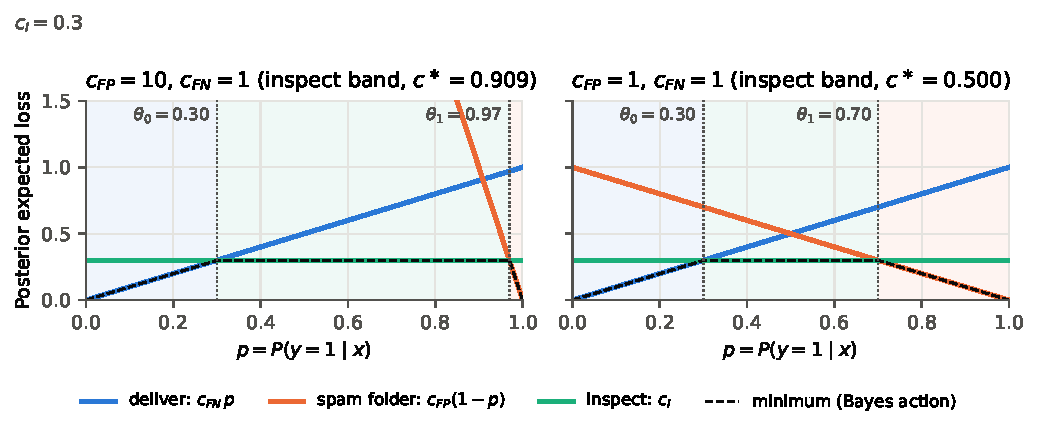
\includegraphics[width=\linewidth]{../project4/figures/t1_expected_loss.pdf}
\caption{Expected loss of each action against $\post$, with $\ci=0.3$. Shading shows where each action
is optimal. Left: our costs $\cfp=10$, $\cfn=1$, inspect band $(0.3,\,0.97)$. Right: equal costs
$\cfp=\cfn=1$, band $(0.3,\,0.7)$, symmetric about $\tstar=1/2$.
Generated by \texttt{experiments/t1\_expected\_loss.py}.}
\label{fig:t1-loss}
\end{figure}

\noindent These thresholds assume $\post$ is the true posterior; a model's estimate gives the Bayes
action only if it is calibrated (Section~\ref{sec:calibration}). The code implements
\eqref{eq:thresholds} in \texttt{decision.bayes\_action}, and a unit test checks it against a direct
minimisation over the three actions on $10{,}000$ random posteriors and loss matrices.

\subsection{The inspection assumption}
\label{sec:inspection}

So far inspection costs $\ci$ whatever the true label, and the inspector always finds the true label
and routes the email correctly. That is why the inspect row of Table~\ref{tab:loss} is constant and
its line in Figure~\ref{fig:t1-loss} is flat.

\paragraph{Variant: imperfect inspection.}
Suppose instead that the inspector sends a real email to spam with probability $\varepsilon_0$ and
delivers a spam with probability $\varepsilon_1$. The inspect row becomes
$L(r,0)=\ci+\varepsilon_0\cfp$ and $L(r,1)=\ci+\varepsilon_1\cfn$, so
$R(r\mid x)=\ci+\varepsilon_0\cfp(1-\post)+\varepsilon_1\cfn\,\post$ is a sloped line rather than a
flat one. It meets the delivery and spam-folder lines at
\[
  \thz' = \frac{\ci+\varepsilon_0\cfp}{(1-\varepsilon_1)\cfn+\varepsilon_0\cfp},
  \qquad
  \tho' = \frac{(1-\varepsilon_0)\cfp-\ci}{(1-\varepsilon_0)\cfp+\varepsilon_1\cfn}.
\]
For $\varepsilon_0=\varepsilon_1=0$ these are $\thz$ and $\tho$. Whenever the band exists
($\ci<\cfn$ is then automatic), $\thz'\ge\thz$ and $\tho'\le\tho$: an unreliable inspector is used for
fewer emails. We keep the perfect-inspection assumption in the rest of the report.
    % T1
\input{sections/03_models}             % T2, T3
\input{sections/04_task2_results}      % C3
\input{sections/05_calibration}        % T4, C4
\input{sections/06_prior_shift}        % T5, C5
\section{Accuracy, cost and rejection}
\label{sec:accuracy-cost}

\subsection{An analytic model (T6)}
\label{sec:t6}
% Member 6

To see exactly how accuracy, cost and rejection trade off, we use a model in which every
quantity has a closed form. Let
\[
  y \sim \mathrm{Bernoulli}(\pio), \qquad x \mid y=1 \sim \mathcal N(+\mu, 1), \qquad
  x \mid y=0 \sim \mathcal N(-\mu, 1), \qquad \mu > 0 .
\]
Write $\phi$ and $\Phi$ for the standard normal density and CDF, $\piz = 1-\pio$, and
$\lambda = \log(\pio/\piz)$ for the prior log-odds.

\paragraph{Posterior and thresholds on $x$.}
The log-likelihood ratio is
$\log\frac{\phi(x-\mu)}{\phi(x+\mu)} = \tfrac12\big[(x+\mu)^2 - (x-\mu)^2\big] = 2\mu x$, so
\begin{equation}
  \post(x) = \Prob(y=1\mid x) = \sigm(2\mu x + \lambda),
  \qquad
  \frac{\pio\,\phi(x-\mu)}{\piz\,\phi(x+\mu)} = e^{2\mu x+\lambda} = \frac{\post(x)}{1-\post(x)} .
  \label{eq:t6-post}
\end{equation}
Since $\post(x)$ is strictly increasing in $x$, the probability threshold $t$ corresponds to the
threshold
\begin{equation}
  x_t = \frac{\logit t - \lambda}{2\mu}
  \label{eq:t6-xt}
\end{equation}
on $x$ ($x_0=-\infty$, $x_1=+\infty$). Every rule ``deliver if $\post\le\thz$, spam if
$\post\ge\tho$, inspect in between'' is therefore the rule ``deliver if $x\le\tau_0$, spam if
$x\ge\tau_1$, inspect in between'' with $\tau_k = x_{\theta_k}$. A two-action rule is the case
$\tau_0=\tau_1=\tau$.

\paragraph{Closed forms.}
For a rule $(\tau_0,\tau_1)$ the probability of each action given each label is
\begin{center}
\begin{tabular}{lccc}
\toprule
 & deliver & spam folder & inspect \\
\midrule
$y=0$ & $\Phi(\tau_0+\mu)$ & $\Phi(-\tau_1-\mu)$ & $\Phi(\tau_1+\mu)-\Phi(\tau_0+\mu)$ \\
$y=1$ & $\Phi(\tau_0-\mu)$ & $\Phi(\mu-\tau_1)$  & $\Phi(\tau_1-\mu)-\Phi(\tau_0-\mu)$ \\
\bottomrule
\end{tabular}
\end{center}
Weighting the rows by $\piz$ and $\pio$ gives the population confusion matrix, and from it
\begin{align}
  \rej(\tau_0,\tau_1) &= \piz\big[\Phi(\tau_1+\mu)-\Phi(\tau_0+\mu)\big]
                        + \pio\big[\Phi(\tau_1-\mu)-\Phi(\tau_0-\mu)\big], \label{eq:t6-rho}\\
  R(\tau_0,\tau_1)    &= \cfp\,\piz\,\Phi(-\tau_1-\mu) + \cfn\,\pio\,\Phi(\tau_0-\mu) + \ci\,\rej(\tau_0,\tau_1),
                        \label{eq:t6-cost}\\
  \mathrm{Acc}(\tau_0,\tau_1) &= \frac{\piz\,\Phi(\tau_0+\mu) + \pio\,\Phi(\mu-\tau_1)}{1-\rej(\tau_0,\tau_1)} .
                        \label{eq:t6-acc}
\end{align}
Here $\rej$ is the rejection (inspection) rate, $R$ the expected cost per email, and
$\mathrm{Acc}$ the accuracy on the emails that were not inspected. For a two-action rule
$\rej=0$ and $\mathrm{Acc}(\tau) = \piz\Phi(\tau+\mu)+\pio\Phi(\mu-\tau)$.

\emph{Check against Section 2.} Differentiating \eqref{eq:t6-cost} and using \eqref{eq:t6-post},
\begin{align*}
  \frac{\partial R}{\partial \tau_1} &= \piz\phi(\tau_1+\mu)\Big[-(\cfp-\ci) + \ci\, e^{2\mu\tau_1+\lambda}\Big], &
  \frac{\partial R}{\partial \tau_0} &= \piz\phi(\tau_0+\mu)\Big[(\cfn-\ci)\,e^{2\mu\tau_0+\lambda} - \ci\Big].
\end{align*}
Each bracket changes sign once, from negative to positive. So $R$ is minimised where the posterior
odds equal $(\cfp-\ci)/\ci$ and $\ci/(\cfn-\ci)$, that is at $\post=1-\ci/\cfp=\tho$ and
$\post=\ci/\cfn=\thz$. These are the thresholds of Section~2, found here without using the
pointwise argument. (This needs $\thz<\tho$, i.e.\ $\ci<\cstar$; otherwise the optimum is a
two-action rule.)

\subsubsection*{Higher accuracy can mean higher cost}

\begin{proposition}\label{prop:acc-cost}
Let $\tau_{\mathrm{acc}} = x_{1/2} = -\lambda/(2\mu)$ and $\tau_{c} = x_{\tstar}$ with
$\tstar = \cfp/(\cfp+\cfn)$. Among two-action rules, $\tau_{\mathrm{acc}}$ uniquely maximises
accuracy and $\tau_c$ uniquely minimises cost. If $\cfp\neq\cfn$ then $\tau_{\mathrm{acc}}\neq\tau_c$,
and for any two thresholds $\tau<\tau'$ in the closed interval between them, the one nearer
$\tau_{\mathrm{acc}}$ has strictly higher accuracy \emph{and} strictly higher cost. In particular the
accuracy-optimal rule is more accurate but more expensive than the cost-optimal rule.
\end{proposition}

\begin{proof}
Using \eqref{eq:t6-post},
\[
  \mathrm{Acc}'(\tau) = \piz\phi(\tau+\mu)\big[1 - e^{2\mu\tau+\lambda}\big], \qquad
  R'(\tau) = \piz\phi(\tau+\mu)\big[\cfn e^{2\mu\tau+\lambda} - \cfp\big].
\]
The factor $\piz\phi(\tau+\mu)$ is positive and $e^{2\mu\tau+\lambda}$ is strictly increasing. So
$\mathrm{Acc}$ strictly increases up to the root $e^{2\mu\tau+\lambda}=1$ (posterior $\tfrac12$,
$\tau=\tau_{\mathrm{acc}}$) and strictly decreases after it. Likewise $R$ strictly decreases up to
$e^{2\mu\tau+\lambda}=\cfp/\cfn$ (posterior $\tstar$, $\tau=\tau_c$) and strictly increases after it.
If $\cfp\ne\cfn$ then $\tstar\ne\tfrac12$ and, as $x_t$ is strictly increasing, $\tau_c\ne\tau_{\mathrm{acc}}$.
Suppose $\cfp>\cfn$, so $\tau_{\mathrm{acc}}<\tau_c$. On $[\tau_{\mathrm{acc}},\tau_c]$, $\mathrm{Acc}$ is
strictly decreasing and $R$ is strictly decreasing, so moving from $\tau$ towards $\tau_c$ lowers both.
The case $\cfp<\cfn$ is symmetric.
\end{proof}

So between the two optima, accuracy and cost always rank rules in \emph{opposite} order: picking
the more accurate of two rules always picks the more expensive one. With $\mu=1$, $\pio=0.4$,
$\cfp=10$, $\cfn=1$ and $\ci=0.3$, Table~\ref{tab:t6} gives the numbers. The accuracy rule is the
most accurate two-action rule, at $84.6\%$, yet it costs $0.772$ per email. That is more than twice the
cost-optimal rule ($0.311$), and also more than the trivial rule that never sends anything to spam
($60\%$ accuracy, cost $0.400$). Figure~\ref{fig:t6-acc-cost} shows both curves against the
probability threshold.

\begin{table}[ht]
\centering\small
\input{\resultsdir/t6_rule_comparison.tex}
\caption{Analytic model with $\mu=1$, $\pio=0.4$, $\cfp=10$, $\cfn=1$, $\ci=0.3$. Accuracy is on
non-inspected emails; FPR $=\Prob(\text{spam folder}\mid y=0)$, FNR $=\Prob(\text{deliver}\mid y=1)$.
Generated by \texttt{experiments/t6\_analytic.py}.}
\label{tab:t6}
\end{table}

\begin{figure}[ht]
\centering
\includegraphics[width=\linewidth]{t6_accuracy_vs_cost.pdf}
\caption{Accuracy and expected cost of the two-action rule ``spam iff $\post\ge t$'' in the analytic
model. Accuracy peaks at $t=0.5$, while cost is lowest at $\tstar=10/11$.}
\label{fig:t6-acc-cost}
\end{figure}

\subsubsection*{Bayes risk as a function of the inspection cost}

The next result holds for any model with calibrated posteriors, not only the Gaussian one. Let
\[
  m(x) = \min\{\cfn\,\post(x),\ \cfp\,(1-\post(x))\}
\]
be the posterior expected loss of the better automatic action. By Section~2 the Bayes action
inspects exactly when $\ci < m(x)$, so the Bayes risk and the rejection rate are
\begin{equation}
  \Rstar(\ci) = \E\big[\min\{m(x),\,\ci\}\big], \qquad \rej(\ci) = \Prob\big(m(x) > \ci\big).
  \label{eq:t6-bayes-risk}
\end{equation}
Write $\Rtwo = \E[m(x)]$ for the Bayes risk without inspection and
$\cstar = \cfp\cfn/(\cfp+\cfn)$.

\begin{lemma}\label{lem:mmax}
$m(x)\le\cstar$ for every $x$, with equality iff $\post(x)=\tstar$.
\end{lemma}
\begin{proof}
$\cfn p$ increases and $\cfp(1-p)$ decreases in $p$. Their minimum is therefore largest where
they are equal, at $p=\cfp/(\cfp+\cfn)=\tstar$, where both equal $\cstar$.
\end{proof}

\begin{proposition}\label{prop:risk-ci}
\begin{enumerate}[label=(\roman*),itemsep=1pt]
  \item $\Rstar$ is non-decreasing and concave on $[0,\infty)$, with $\Rstar(0)=0$.
  \item Its right derivative is $\rej(\ci)$. Wherever $\Prob(m(x)=\ci)=0$ (for every $\ci$ in the Gaussian
        model), $\Rstar$ is differentiable with $\frac{d\Rstar}{d\ci} = \rej(\ci)$, and $\rej$ is
        non-increasing.
  \item Rejection stops at $\cstar$: $\rej(\ci)=0$ and $\Rstar(\ci)=\Rtwo$ for all $\ci\ge\cstar$.
  \item $\Rtwo-\Rstar(\ci)=\int_{\ci}^{\cstar}\rej(s)\,ds$. In the Gaussian model this is strictly
        positive iff $\ci<\cstar$, so allowing inspection improves the system iff $\ci<\cstar$.
\end{enumerate}
\end{proposition}

\begin{proof}
(i) For each fixed $x$, $c\mapsto\min\{m(x),c\}$ is the minimum of two non-decreasing affine
functions of $c$, so it is non-decreasing and concave. Both properties survive taking the expectation.
At $c=0$ the minimum is $0$ because $m\ge0$.

(ii) For $h>0$,
$\frac1h\big[\min\{m,c+h\}-\min\{m,c\}\big]$ lies in $[0,1]$ and tends to $\mathbf 1\{m>c\}$ as
$h\downarrow0$. By dominated convergence the right derivative of $\Rstar$ is $\Prob(m>c)=\rej(c)$.
The left derivative is, in the same way, $\Prob(m\ge c)$, and the two agree when $\Prob(m=c)=0$.
In the Gaussian model $\post(x)$ is strictly monotone in $x$, so $\{x: m(x)=c\}$ has at most
two points and probability zero. $\rej$ is non-increasing because $\{m>c'\}\subseteq\{m>c\}$ for
$c'>c$. This is a second proof of concavity.

(iii) By Lemma~\ref{lem:mmax}, $m(x)\le\cstar\le\ci$, so $\rej(\ci)=\Prob(m>\ci)=0$ and
$\min\{m,\ci\}=m$, giving $\Rstar(\ci)=\E[m]=\Rtwo$.

(iv) By (ii) and (iii), $\Rtwo-\Rstar(\ci)=\Rstar(\cstar)-\Rstar(\ci)=\int_{\ci}^{\cstar}\rej(s)\,ds$.
In the Gaussian model $\post(x)$ takes every value in $(0,1)$. For $s<\cstar$ the set
$\{x: m(x)>s\}=\{x:\thz(s)<\post(x)<\tho(s)\}$ is a non-empty open interval of $x$, so
$\rej(s)>0$. The integral is therefore positive iff $\ci<\cstar$.
\end{proof}

Proposition~\ref{prop:risk-ci} says three things. First, the rejection rate is the marginal cost
of inspection: raising $\ci$ by a small $\delta$ raises the Bayes risk by $\rej\,\delta$, because only the
inspected emails pay the extra cost. Second, the saving from allowing inspection is the area under
the rejection curve to the right of $\ci$. Third, inspection is worth paying for exactly when it is
cheaper than the worst-case automatic loss $\cstar$. With $\cfp=10$ and $\cfn=1$ that cut-off
is $\cstar=10/11\approx0.909$, and it does not depend on $\mu$ or $\pio$.
Because these results hold for every $\ci$, the price $\ci=0.3$ of Section~\ref{sec:loss-matrix} serves
only as a representative value for tables: it lies well below $\cstar$, so inspection is used, and any
other price below $\cstar$ leads to the same conclusions.
In the Gaussian model the curves follow in closed form: put $\tau_k=x_{\theta_k(\ci)}$ from
\eqref{eq:t6-xt} into \eqref{eq:t6-rho} and \eqref{eq:t6-cost}. Figure~\ref{fig:t6-risk} plots them for
three class separations. Better-separated classes have lower risk at every $\ci$, and all three
curves stop rejecting at the same $\cstar$. The rejection rate, however, is not ordered by $\mu$:
weakly separated classes ($\mu=0.5$) inspect more emails than $\mu=1$ when inspection is cheap, but
fewer once $\ci\gtrsim0.57$. With weak separation most posteriors stay close to the prior $0.4$.
Once the lower threshold $\thz=\ci/\cfn$ climbs past them, those emails are delivered rather than
inspected. (For $\mu=0.5$ the best two-action rule is almost ``always deliver'': $\Rtwo=0.399$
against $\pio\cfn=0.4$.) At the default $\ci=0.3$
with $\mu=1$, inspecting $41.6\%$ of emails cuts the cost from $\Rtwo=0.311$ to $0.179$.

\begin{figure}[ht]
\centering
\includegraphics[width=\linewidth]{t6_risk_reject_vs_cinsp.pdf}
\caption{Analytic Bayes risk $\Rstar(\ci)$ and rejection rate $\rej(\ci)$ for $\pio=0.4$,
$\cfp=10$, $\cfn=1$ and three separations $\mu$. Dotted lines show $\Rtwo$, the best risk without
inspection. Rejection falls to zero at $\cstar=10/11$ (dashed), after which $\Rstar=\Rtwo$.}
\label{fig:t6-risk}
\end{figure}

\begin{assumptions}
One-dimensional equal-variance Gaussian classes with known $\mu$ and $\pio$, so the posterior is
exact (calibrated); zero loss for correct decisions; constant inspection cost $\ci$ and a perfect
inspector. Lemma~\ref{lem:mmax} and Proposition~\ref{prop:risk-ci}(i)--(iii) need only calibrated
posteriors and this loss matrix. Part (iv) and Proposition~\ref{prop:acc-cost} use the Gaussian model.
\end{assumptions}

\emph{Numerical check.} \texttt{tests/test\_analytic.py} draws $400{,}000$ samples from the model,
applies the Bayes rule, and confirms that the realized loss, rejection rate and accuracy match
\eqref{eq:t6-rho}--\eqref{eq:t6-acc}. It also checks that a grid search over all rules
$(\tau_0,\tau_1)$ never beats the Bayes thresholds, and that a finite-difference slope of
$\Rstar$ equals $\rej$.

\subsection{Experiments (C6)}
\label{sec:c6}
For split $s=0,\ldots,19$ we drew $10{,}000$ Gaussian messages ($\mu=1$, $\pio=0.4$,
seed $10{,}000+s$) and split the Spambase corpus using the same stratified $60/20/20$ protocol.
We standardized features and fitted models on training data. Validation log-loss selected
the shared-covariance Gaussian shrinkage from the team's grid and the logistic penalty from
$0.01,0.1,1,10,100$. Each fitted model used identical test predictions across rules and prices.
Tables and bands give means and one standard error over splits. Overlapping Spambase test sets
make these bands descriptive of split variability.

\begin{table}[htbp]
\centering\small
\input{\resultsdir/c6_rules.tex}
\caption{Two automatic rules on held-out messages. Accuracy is the fraction of all test
messages classified correctly. Cost is realized loss per message at $\cfp=10,\cfn=1$.}
\label{tab:c6-rules}
\end{table}

On synthetic data, changing the Gaussian rule from $0.5$ to $10/11$ lowered accuracy
from $84.6\%$ to $73.9\%$ and more than halved its cost (Table~\ref{tab:c6-rules}).
At ten times the price of a missed spam email, avoiding one false positive pays for up to
ten extra false negatives. Both fitted models show the same accuracy--cost ordering
on Spambase.

\begin{table}[htbp]
\centering\small
\input{\resultsdir/c6_savings.tex}
\caption{Inspection at $\ci=0.3$. The two-action baseline uses each fitted posterior at
$\tstar=10/11$. Costs and paired savings are per email. The last column is the fraction inspected.}
\label{tab:c6-savings}
\end{table}

\begin{figure}[htbp]
\centering
\includegraphics[width=0.88\linewidth]{c6_inspection_synthetic.pdf}
\caption{Synthetic held-out results against the exact risk and rejection rate for the
true Gaussian posterior. Narrow bands and overlapping lines reflect close agreement.
The vertical line marks $\cstar=10/11$.}
\label{fig:c6-synthetic}
\end{figure}
\begin{figure}[htbp]
\centering
\includegraphics[width=0.88\linewidth]{c6_inspection_spambase.pdf}
\caption{Spambase held-out cost and inspection rate. At and above the marked cutoff both
models take only automatic actions, so each cost curve levels off at its own baseline.}
\label{fig:c6-spambase}
\end{figure}

At $\ci=0.3$ theory predicts cost $0.179$ and rejection $0.416$. The fitted Gaussian
gives $0.181$ and $0.417$ (Figure~\ref{fig:c6-synthetic}). On Spambase the logistic fit
saves $0.100$ per email while inspecting $24.1\%$ (Figure~\ref{fig:c6-spambase} and Table~\ref{tab:c6-savings}).
At zero price, both models inspected every test email on both datasets, with zero realized
cost in every split. A finite fitted log-odds score implies a probability strictly between
zero and one. Comparing scores directly with the log-odds thresholds preserves this fact
even for forecasts that would round to an endpoint in probability space.

For a true posterior the gain over the best two-action rule is
$\Rtwo-\Rstar(\ci)=\E[(m(X)-\ci)_+]$, where $u_+=\max(u,0)$.
It is strictly positive exactly when $\Prob(m(X)>\ci)>0$. Every nonempty inspection
band has positive probability in the Gaussian model. On Spambase the true posterior is unknown,
so the table compares the fitted policies on observed labels.

\paragraph{Sensitivity to repeated feature vectors.}
About $9.8\%$ of Spambase test rows had an exact 57-feature match in their training split.
Excluding those rows preserved the conclusion: inspection reduced logistic cost from
$0.264$ to $0.160$ and Gaussian cost from $0.291$ to $0.173$ per email.
 % T6, C6
\input{sections/08_conclusion}         % one paragraph per member

\appendix
\input{sections/A_contributions}

\bibliographystyle{plain}
\bibliography{references}
\end{document}
